%% ----------------------------------------------------------------------------------
%% GUIDELINES
%% ----------------------------------------------------------------------------------
%% - Provide details about techniques/methods that you use. Do not just write “We have
%% implemented the marching cubes algorithm”. Describe the method too, in your own
%% words. Even if it is well described in a book, you should still explain the method
%% yourself; this is part of the exercise. Also, the reader may not know the method, nor
%% can the reader be bothered to find the document that you are referring to.
%% - Discuss interesting implementation aspects, but do not include code fragments in the
%% text. Pseudo code is allowed, but mathematical formulas are preferred.
%% - Describe parameters of methods and explain which settings you used and why.
%% - Provide evidence that the method you have implemented actually works as intended.
%% - Explain how you designed a color map, a transfer function, or even your whole visualization
%% approach.

\todo { user controls!! user existing controls.. extra radio box }

\section{Opacity Weighting}\label{sec:opacity}

\subsection{Comparison with Compositing}\label{subsec:opacity_compare}

- Opacity shows volumes, tries to find the edges
- Both show multiple layers
- Opacity clearly shows the structure of the piggy bank (REF), shows the borders of the material
- also the flowers are pretty visible, specially in comparison with composition



\begin{figure}[h!]
    \centering
    \captionsetup{justification=centering,margin=0.5cm}
    \begin{subfigure}[t]{0.49\textwidth}
        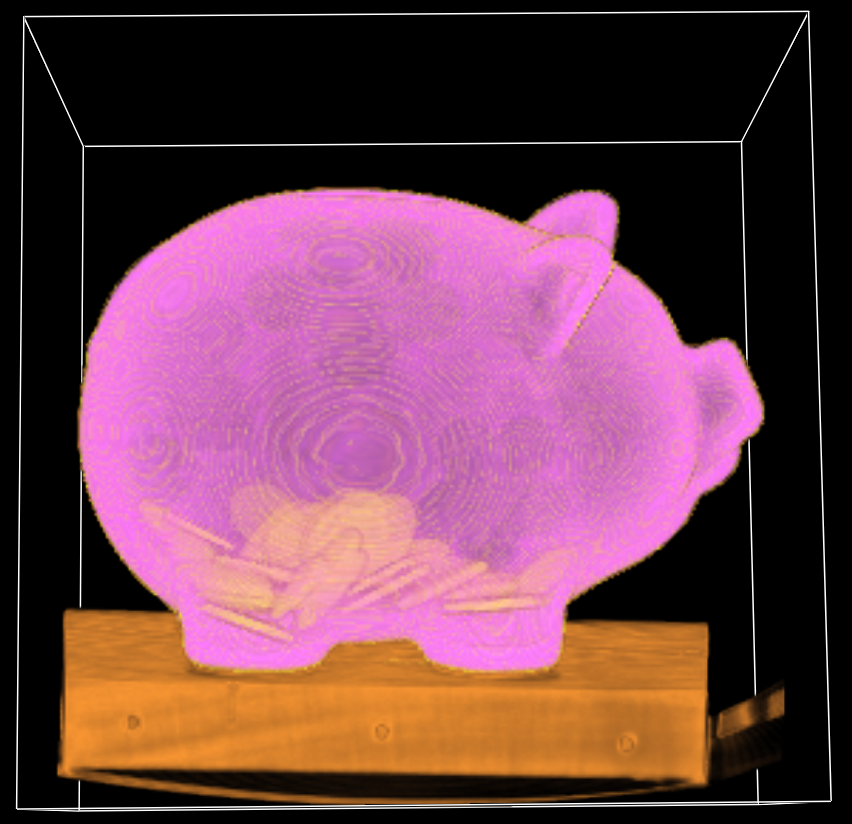
\includegraphics[width=\textwidth]{img/pig-compositing.png}
        \caption{ }
    \end{subfigure}
    \begin{subfigure}[t]{0.49\textwidth}
        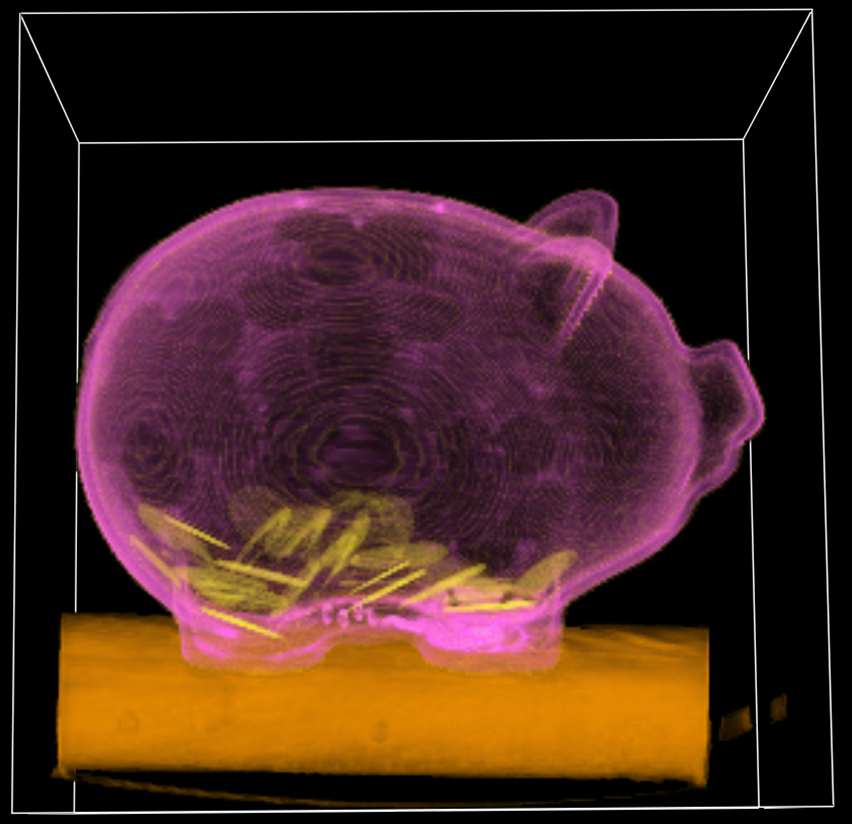
\includegraphics[width=\textwidth]{img/pig-opacity.png}
        \caption{ }
    \end{subfigure}
    \caption{(a) Rendering with compositing raycaster, (b) rendering with opacity weighting raycaster}
    \label{fig:compareraycasters}
\end{figure}


\begin{figure}[h!]
    \centering
    \captionsetup{justification=centering,margin=0.5cm}
    \begin{subfigure}[t]{0.32\textwidth}
        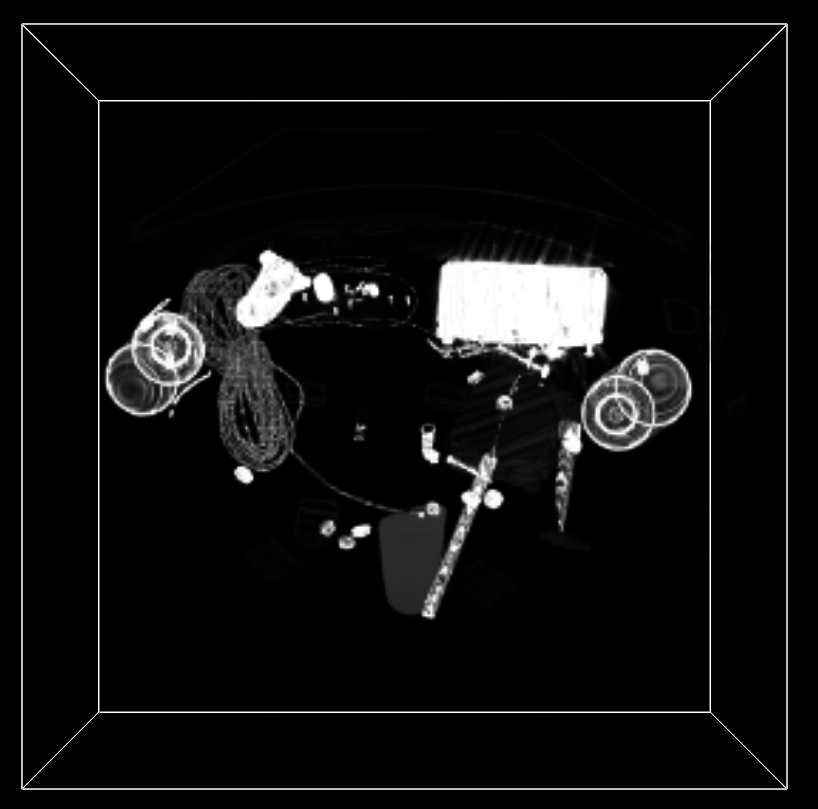
\includegraphics[width=\textwidth]{img/bag-MIP.png}
        \caption{ }
    \end{subfigure}
    \begin{subfigure}[t]{0.32\textwidth}
        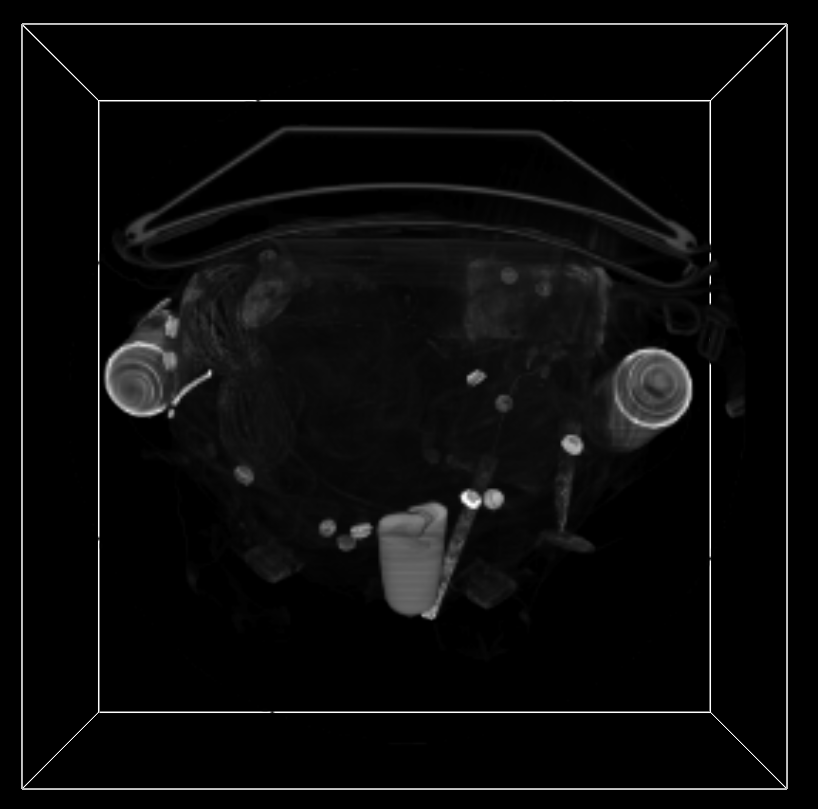
\includegraphics[width=\textwidth]{img/bag-Composition.png}
        \caption{ }
    \end{subfigure}
    \begin{subfigure}[t]{0.32\textwidth}
        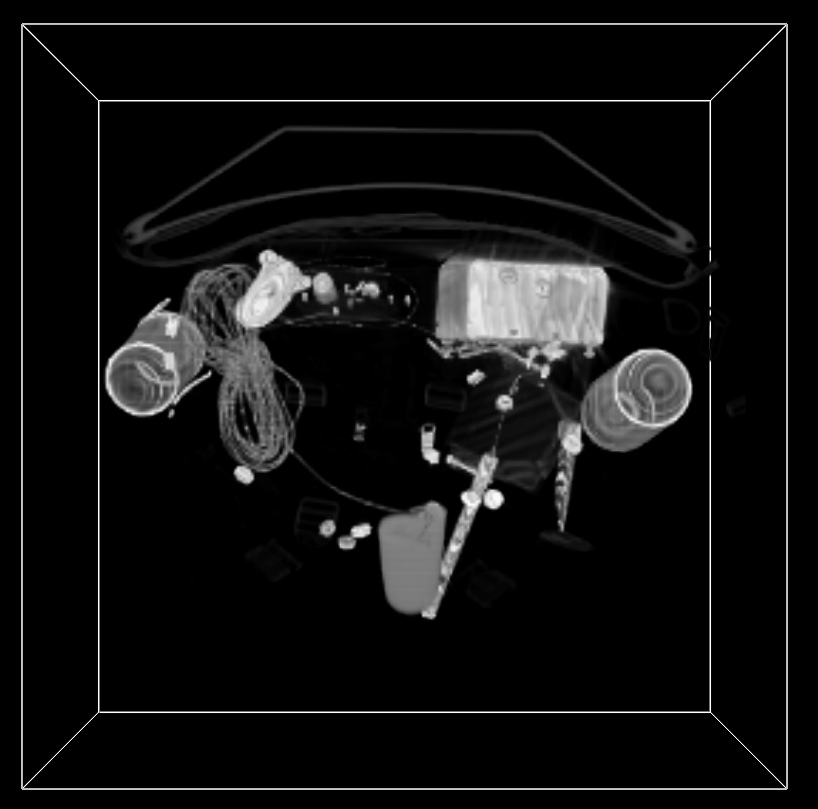
\includegraphics[width=\textwidth]{img/bag-Opacity.png}
        \caption{ }
    \end{subfigure}
    \caption{(a) Rendering with MIP raycaster, (a) Rendering with compositing raycaster, (b) rendering with opacity weighting raycaster}
    \label{fig:compareraycasters}
\end{figure}